\documentclass[14pt]{extbook}
\usepackage{multicol, enumerate, enumitem, hyperref, color, soul, setspace, parskip, fancyhdr} %General Packages
\usepackage{amssymb, amsthm, amsmath, latexsym, units, mathtools} %Math Packages
\everymath{\displaystyle} %All math in Display Style
% Packages with additional options
\usepackage[headsep=0.5cm,headheight=12pt, left=1 in,right= 1 in,top= 1 in,bottom= 1 in]{geometry}
\usepackage[usenames,dvipsnames]{xcolor}
\usepackage{dashrule}  % Package to use the command below to create lines between items
\newcommand{\litem}[1]{\item#1\hspace*{-1cm}\rule{\textwidth}{0.4pt}}
\pagestyle{fancy}
\lhead{Makeup Progress Quiz 2}
\chead{}
\rhead{Version C}
\lfoot{2790-1423}
\cfoot{}
\rfoot{Summer C 2021}
\begin{document}

\begin{enumerate}
\litem{
Choose the equation of the function graphed below.
\begin{center}
    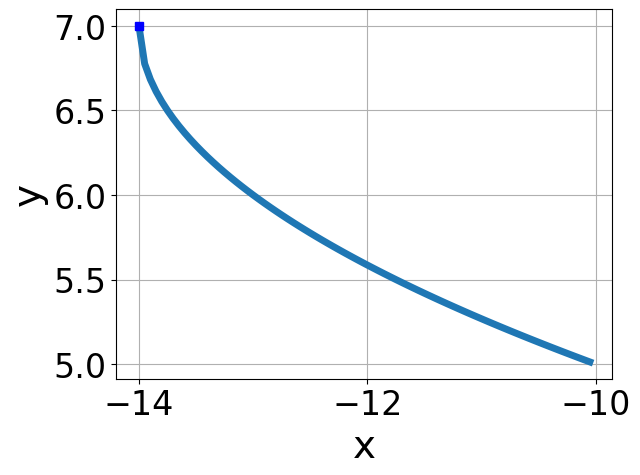
\includegraphics[width=0.5\textwidth]{../Figures/radicalGraphToEquationCopyC.png}
\end{center}
\begin{enumerate}[label=\Alph*.]
\item \( f(x) = - \sqrt[3]{x + 14} + 7 \)
\item \( f(x) = \sqrt[3]{x + 14} + 7 \)
\item \( f(x) = \sqrt[3]{x - 14} + 7 \)
\item \( f(x) = - \sqrt[3]{x - 14} + 7 \)
\item \( \text{None of the above} \)

\end{enumerate} }
\litem{
What is the domain of the function below?\[ f(x) = \sqrt[8]{-7 x + 3} \]\begin{enumerate}[label=\Alph*.]
\item \( (-\infty, \infty) \)
\item \( (-\infty, a], \text{ where } a \in [0, 2] \)
\item \( [a, \infty), \text{where } a \in [1.4, 5.4] \)
\item \( [a, \infty), \text{where } a \in [-1.9, 0.8] \)
\item \( (-\infty, a], \text{where } a \in [1.8, 4.7] \)

\end{enumerate} }
\litem{
Solve the radical equation below. Then, choose the interval(s) that the solution(s) belongs to.\[ \sqrt{35 x^2 + 42} - \sqrt{-79 x} = 0 \]\begin{enumerate}[label=\Alph*.]
\item \( x_1 \in [0.72, 1.71] \text{ and } x_2 \in [0.9,3.5] \)
\item \( \text{All solutions lead to invalid or complex values in the equation.} \)
\item \( x \in [-1.61,-0.88] \)
\item \( x \in [-0.88,-0.84] \)
\item \( x_1 \in [-1.61, -0.88] \text{ and } x_2 \in [-1.2,0.3] \)

\end{enumerate} }
\litem{
Choose the graph of the equation below.\[ f(x) = - \sqrt{x - 6} + 7 \]\begin{enumerate}[label=\Alph*.]
\begin{multicols}{2}\item 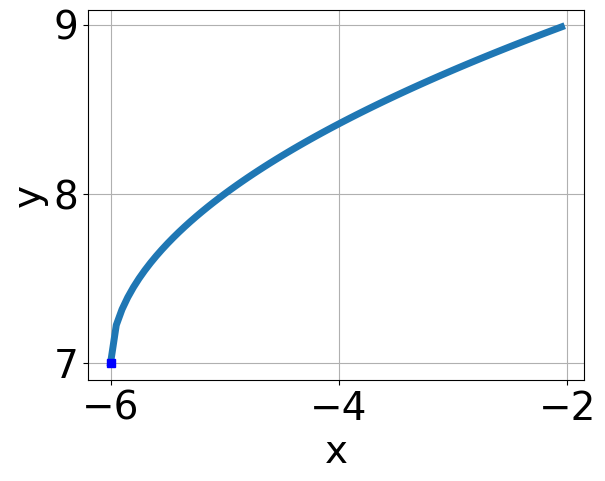
\includegraphics[width = 0.3\textwidth]{../Figures/radicalEquationToGraphAC.png}\item 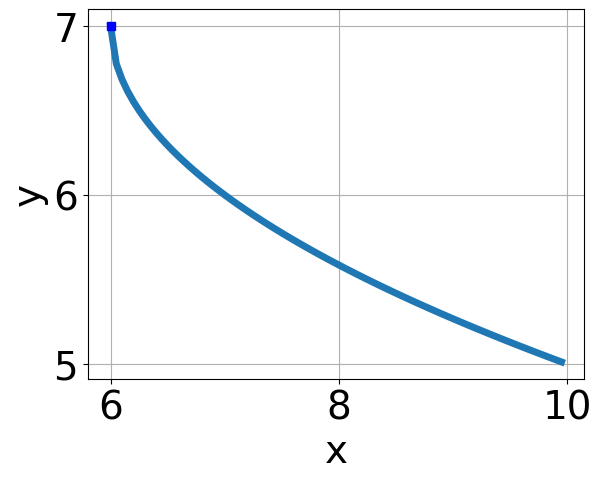
\includegraphics[width = 0.3\textwidth]{../Figures/radicalEquationToGraphBC.png}\item 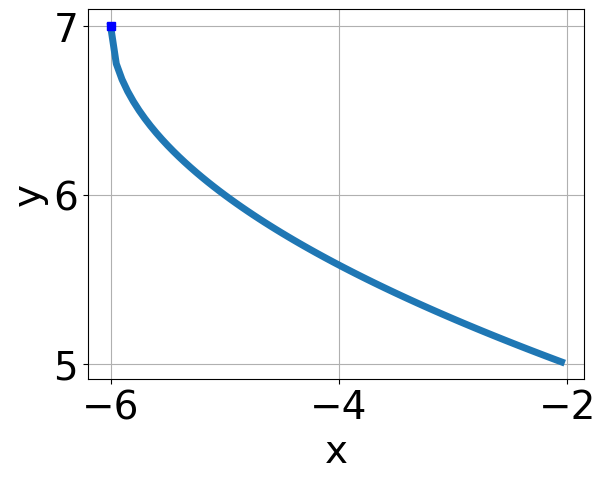
\includegraphics[width = 0.3\textwidth]{../Figures/radicalEquationToGraphCC.png}\item 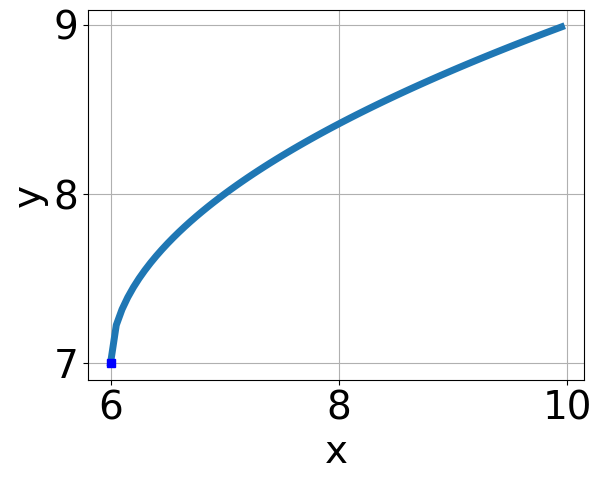
\includegraphics[width = 0.3\textwidth]{../Figures/radicalEquationToGraphDC.png}\end{multicols}\item None of the above.
\end{enumerate} }
\litem{
What is the domain of the function below?\[ f(x) = \sqrt[4]{6 x - 4} \]\begin{enumerate}[label=\Alph*.]
\item \( [a, \infty), \text{ where } a \in [0.51, 1.35] \)
\item \( [a, \infty), \text{where } a \in [1.46, 1.7] \)
\item \( (-\infty, a], \text{where } a \in [1.3, 4.3] \)
\item \( (-\infty, \infty) \)
\item \( (-\infty, a], \text{where } a \in [0.5, 1] \)

\end{enumerate} }
\litem{
Solve the radical equation below. Then, choose the interval(s) that the solution(s) belongs to.\[ \sqrt{-6 x - 5} - \sqrt{2 x + 5} = 0 \]\begin{enumerate}[label=\Alph*.]
\item \( x_1 \in [-2.6, -1.5] \text{ and } x_2 \in [-5.83,1.17] \)
\item \( x \in [-0.7,1.3] \)
\item \( x \in [-2.1,-0.4] \)
\item \( x_1 \in [-2.1, -0.4] \text{ and } x_2 \in [-5.83,1.17] \)
\item \( \text{All solutions lead to invalid or complex values in the equation.} \)

\end{enumerate} }
\litem{
Choose the equation of the function graphed below.
\begin{center}
    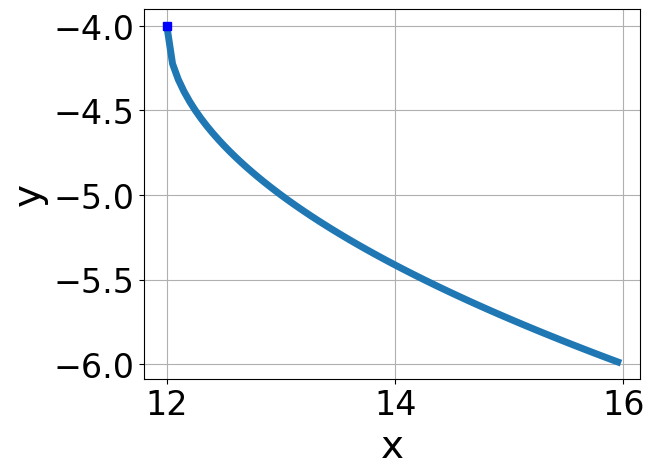
\includegraphics[width=0.5\textwidth]{../Figures/radicalGraphToEquationC.png}
\end{center}
\begin{enumerate}[label=\Alph*.]
\item \( f(x) = \sqrt{x + 12} - 4 \)
\item \( f(x) = - \sqrt{x + 12} - 4 \)
\item \( f(x) = \sqrt{x - 12} - 4 \)
\item \( f(x) = - \sqrt{x - 12} - 4 \)
\item \( \text{None of the above} \)

\end{enumerate} }
\litem{
Solve the radical equation below. Then, choose the interval(s) that the solution(s) belongs to.\[ \sqrt{-9 x^2 - 24} - \sqrt{33 x} = 0 \]\begin{enumerate}[label=\Alph*.]
\item \( x_1 \in [2.58, 3.03] \text{ and } x_2 \in [-0.1,4.2] \)
\item \( x \in [-2.44,-0.68] \)
\item \( x \in [-3.14,-2.26] \)
\item \( x_1 \in [-3.14, -2.26] \text{ and } x_2 \in [-1.4,0.9] \)
\item \( \text{All solutions lead to invalid or complex values in the equation.} \)

\end{enumerate} }
\litem{
Choose the graph of the equation below.\[ f(x) = - \sqrt{x - 12} + 7 \]\begin{enumerate}[label=\Alph*.]
\begin{multicols}{2}\item 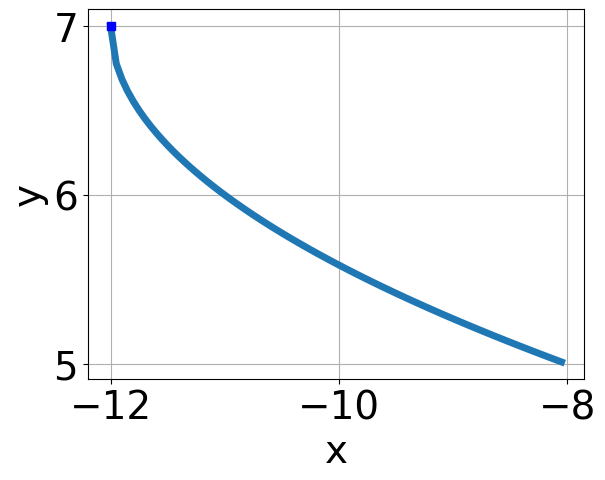
\includegraphics[width = 0.3\textwidth]{../Figures/radicalEquationToGraphCopyAC.png}\item 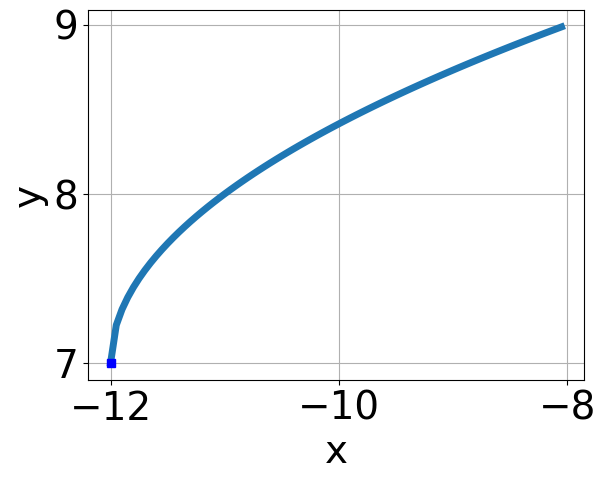
\includegraphics[width = 0.3\textwidth]{../Figures/radicalEquationToGraphCopyBC.png}\item 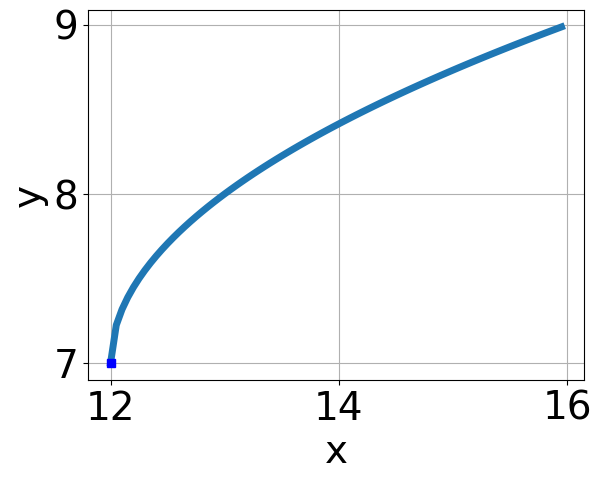
\includegraphics[width = 0.3\textwidth]{../Figures/radicalEquationToGraphCopyCC.png}\item 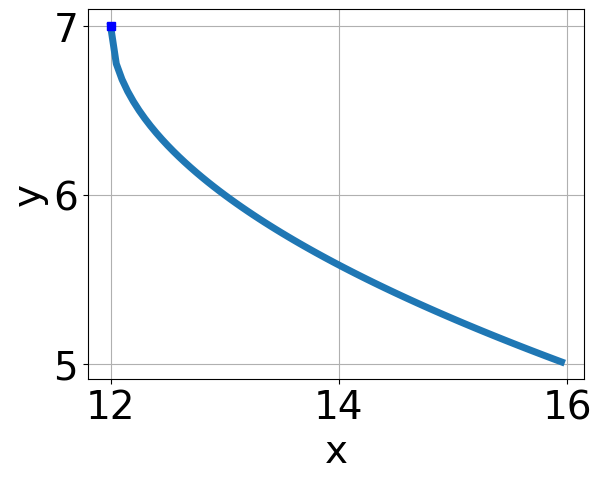
\includegraphics[width = 0.3\textwidth]{../Figures/radicalEquationToGraphCopyDC.png}\end{multicols}\item None of the above.
\end{enumerate} }
\litem{
Solve the radical equation below. Then, choose the interval(s) that the solution(s) belongs to.\[ \sqrt{4 x - 6} - \sqrt{7 x - 4} = 0 \]\begin{enumerate}[label=\Alph*.]
\item \( x_1 \in [-1.08, 0.01] \text{ and } x_2 \in [1.5,3.5] \)
\item \( x \in [-1.08,0.01] \)
\item \( x \in [-3.64,-3.28] \)
\item \( \text{All solutions lead to invalid or complex values in the equation.} \)
\item \( x_1 \in [-0.51, 0.84] \text{ and } x_2 \in [1.5,3.5] \)

\end{enumerate} }
\end{enumerate}

\end{document}